%%%%%%%%%%%%%%%%%%%%%%%%%%%%%%%%%%%%%%%%%%%%%%%%%%%
% msc.tex
%%%%%%%%%%%%%%%%%%%%%%%%%%%%%%%%%%%%%%%%%%%%%%%%%%%
At present, the Monte Carlo simulation of charged particle transport in detailed
(interaction by interaction) mode is feasible only for projectiles with 
relatively low energies and for thin targets.  In general, the number of 
elastic interactions of a projectile before being stopped is very large and
detailed simulation becomes impractical.  The conventional solution for 
overcoming this difficulty is the implementation of condensed-history 
simulation schemes, in which the cumulative effect of many elastic scatterings
along a given track segment is simulated by using multiple scattering theories
such as Moli\`{e}re \cite{embib:msc2, embib:msc3}, Goudsmit and Saunderson
\cite{embib:msc4} and Lewis \cite{embib:msc6}.

\Gfour{} offers a diverse set of multiple scattering and single scattering
models \cite{embib:msc61,embib:msc1,embib:msc8,embib:msc9}.  Multiple scattering
models share the same \gclass{G4VMscModel} interface and were tuned per particle
type and application domain.  Recently, the possibility of sampling the lateral 
displacement of a charged particle at a geometry boundary was achieved by moving
the sampling of particle scattering from post-step to along-step, before 
sampling the energy loss and straggling.

Single scattering models sample each elastic collision of a charged particle, 
resulting in an increased number of steps and increased simulation time in 
comparison to multiple scattering models.  However, single scattering models 
have several important applications.  In particular, they are needed for the 
simulation of recoils \cite{embib:msc8,embib:msc9}, which is crucial, for 
example, for the understanding of single event effects in space electronics. 
Single scattering models are also needed to perform comparisons and validations
of multiple scattering models.  Single scattering models are useful for the 
sampling of charged particle transport in thin layers or low density media, and
in the vicinity of boundary crossing between two volumes.  In the majority of 
benchmark results for all particle types, single scattering predictions are 
closer to reference data than those of multiple scattering.

The choice of multiple scattering model strongly influences the CPU 
performance of the EM simulation.  The new unified design \cite{bib:uni} allows 
different multiple scattering models for different energy ranges to be used 
within the same simulation.  The analysis of all available results from multiple
scattering benchmarks \cite{embib:chep11,embib:msc1,embib:chep12} 
allows establishment of the optimal configuration of multiple and single 
scattering models in production physics lists.

In default physics lists, the Urban model is used below 100 MeV for electrons 
and positrons, where this model has a significant advantage in accuracy and 
CPU speed.  In the combined model \gclass{G4WentzelVIModel}, single scattering 
is applied only for hard scattering, which has a limited cross section, while
small angle scattering is sampled as multiple scattering \cite{embib:msc1}. 
The \gclass{G4WentzelVIModel} model provides results similar in accuracy to 
single scattering but it is much more computationally efficient.  As such, 
recent versions of \Gfour{} have this combined model set as the default for muon
and hadron transport, and for $e^{\pm}$ above 100 MeV.  Validation of multiple
scattering models for muons and hadrons are published elsewhere 
\cite{embib:chep14,embib:chep11,embib:msc1,embib:msc12}.

As an example of benchmark tests carried out, Figure~\ref{Figure-MSC1} 
illustrates the ratios of simulated to measured angular distribution widths
taken at the points where the distrubution falls to 1/e of the peak value.  The
measured data taken from literature \cite{embib:msc11} include a set of 
different target materials (Be, C, Al, Ti, Cu, Ta, Au) with an accuracy of about
1\%.  Using the \gclass{G4UrbanMscModel} of \Gfour{} release 10.0, the predicted 
angular distribution widths are close to the data with a maximum deviation not 
exceeding 3\% for both test cases of 13 and 20 MeV. 

\begin{figure}
\includegraphics[width=0.5\textwidth]{figures/ratio_13.pdf}
% \includegraphics[width=0.5\textwidth]{electromagnetic/ratio_13.eps}
\caption{The MC/data ratio of angular distribution widths measured at the 1/e
level for the Urban model of \Gfour{} 10.0.  Results are shown for a 13~MeV beam
on the target materials and thicknesses of the electron scattering benchmark
\cite{embib:msc11} .}
\label{Figure-MSC1}
\end{figure}


